\documentclass{article}
\usepackage{graphics}
\usepackage{indentfirst}
\usepackage{amsmath}
\usepackage{algorithm}
\usepackage{algorithmic}
\usepackage{bm}
\usepackage{setspace}
\usepackage{graphicx}
\usepackage{float}
\author{Ruichen Wang \\
wangrc@2345.com}
\title{Variational Auto Encoder}
\begin{document}
\maketitle
\begin{abstract}
Variational auto-encoder \cite{DBLP:journals/corr/KingmaW13} is a very powful generative model. It can be used to generate or convert videos, images, texts, sounds etc. 
\end{abstract}

\tableofcontents
\section{What is VAE?} 
Variational auto-encoder is a brilliant combination of deep learning and variational inferece. It was proposed by Kingma in 2013. It provides a probabilistic manner for describing an observation in latent space. The encoder is aimed to describe a probability distribution for each latent attribute.
\begin{figure}[h]
\centering
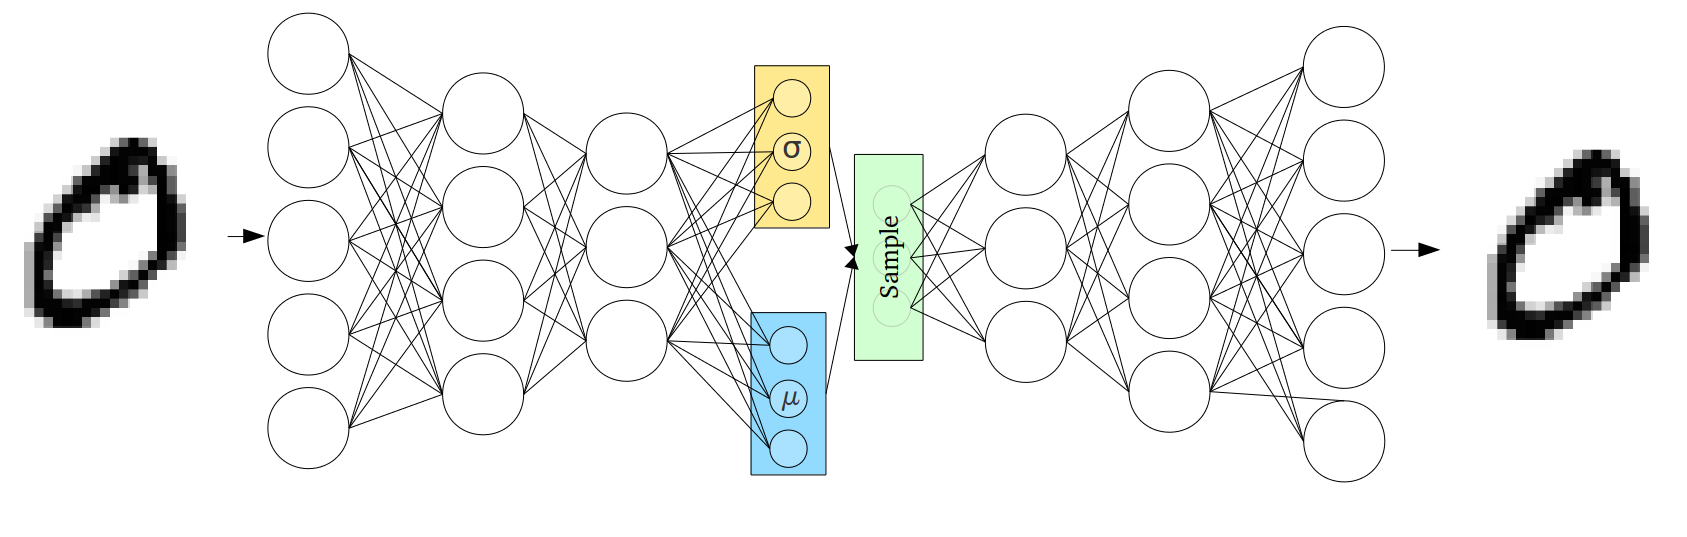
\includegraphics[width=5in,height=1.5in]{graph1}
\caption{VAE graph model}
\end{figure}
\subsection{Intuition}
In the past, we want the encoder to learn some  dimensions of input as the compressed feature. Using a variational autoencoder, we describe those latent dimensions in probabilistic terms.we'll now instead represent each latent attribute for a given input as a probability distribution. And we will perform random sampling on the distirbution to feed the decoder. We expecting the decoder can accurately reconstruct the input.

\subsection{Statisical motivation}
Suppose there exists some latent variable $z$ controls the observation $x$. We would like to infer the posterior $p_{\theta}(z|x)$
\begin{figure}[h]
\centering
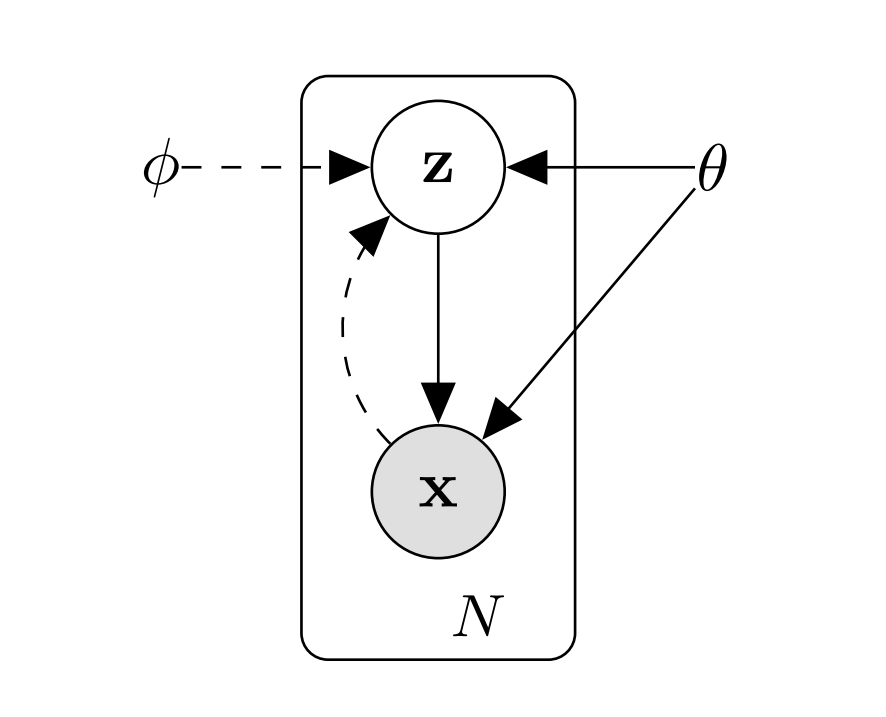
\includegraphics[width=2.5in,height=2in]{graph2}
\caption{Solid lines denotes the generative model $p_{\theta}(z)p_{\theta}(x|z)$. Dash lines denote the variational inference $q_{\phi}(z|x)$ which is a approximation of intractable $p_{\theta}(z|x)$.}
\end{figure}
$$p_{\theta}(z|x)=\frac{p_{\theta}(x|z)p_{\theta}(z)}{p_{\theta}(x)}=\frac{p_{\theta}(x|z)p_{\theta}(z)}{\int p_{\theta}(z)p_{\theta}(x|z)dz}$$

As we \textbf{do not} make the common simplifying assumptions about the marginal or posterior probabilities, the $\int p_{\theta}(z)p_{\theta}(x|z)dz$ is intractable, and EM algorithm or mean-field variational bayesian is also intractable.

So the VAE introduce a recognition model $q_{\phi}(z|x)$, which is a approximation to the posterior. Note the $\phi$ can not be computed from some closed-form expectation like mean-filed variational inference. It will be learned jointly with $\theta$.


\begin{figure}[h]
\centering
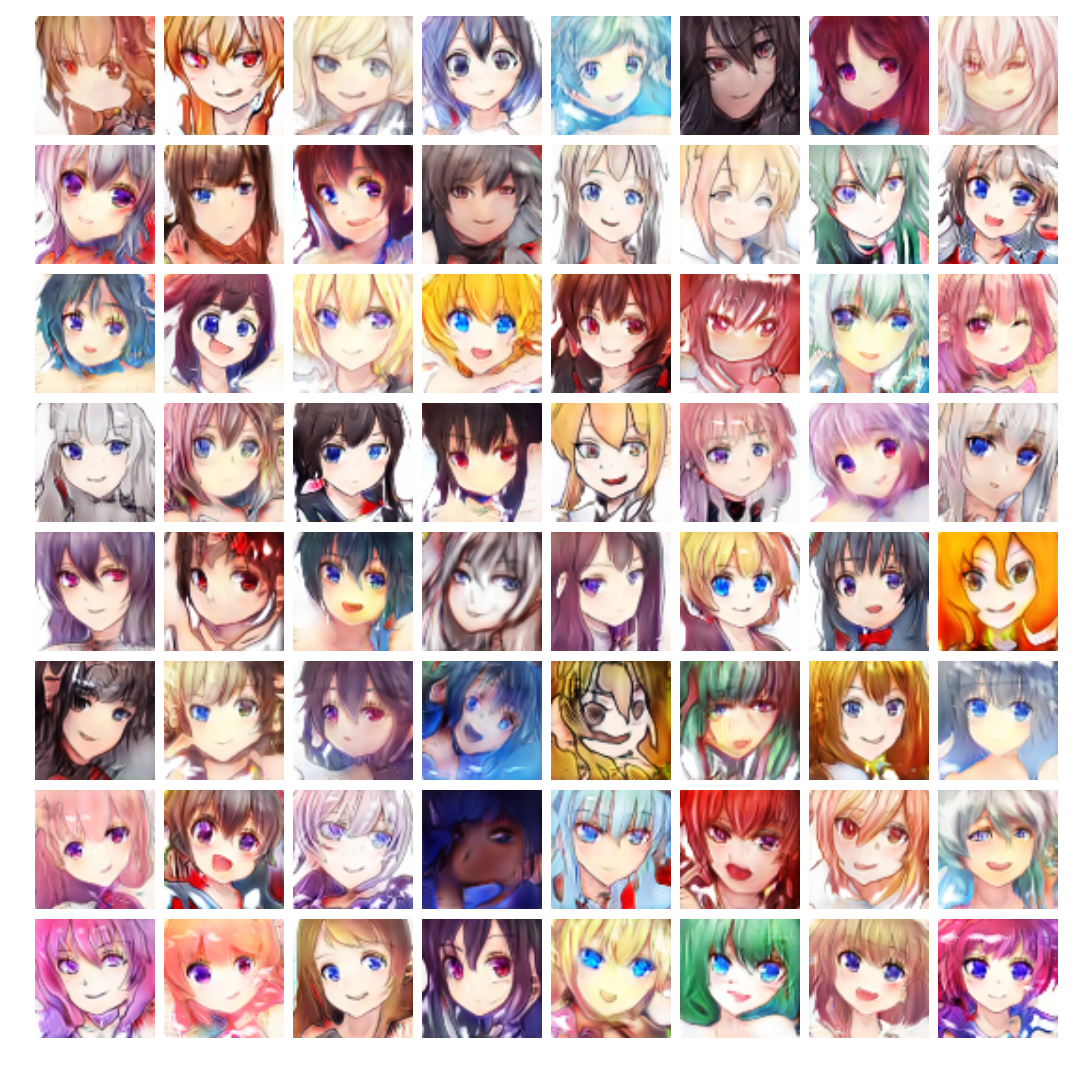
\includegraphics[width=5in,height=5in]{result1}
\caption{Generated images}
\end{figure}


\bibliographystyle{plain}
\bibliography{ref}

\end{document}


























